\documentclass{beamer}
% \documentclass[handout]{beamer}

\usepackage[utf8]{inputenc} 
\usepackage[english]{babel}
\usepackage[acronyms]{glossaries}
\usepackage{color}
\usepackage{listings}
\usepackage{stmaryrd}
\usepackage{bussproofs}
\usepackage{appendixnumberbeamer}
\usetheme[progressbar=frametitle]{metropolis}

%
% TeXiS
%
\def\titulo{Program Verification in Elixir}
\def\autor{Adrián Enríquez Ballester}

%
% Acronyms
%
\newacronym{api}{API}{Application Programming Interface}
\newacronym{ast}{AST}{Abstract Syntax Tree}
\newacronym{csp}{CSP}{Constraint Satisfaction Problem}
\newacronym{dialyzer}{Dialyzer}{DIscrepancy AnaLYZer for ERlang programs}
\newacronym{dsl}{DSL}{Domain Specific Language}
\newacronym{io}{I/O}{Input/Output}
\newacronym{ir}{IR}{Intermediate Representation}
\newacronym{jvm}{JVM}{Java Virtual Machine}
\newacronym{llvm}{LLVM}{Low-Level Virtual Machine}
\newacronym{nif}{NIF}{Native Implemented Function}
\newacronym{oop}{OOP}{Object-oriented programming}
\newacronym{proper}{PropEr}{PROPerty-based testing tool for ERlang}
\newacronym{repl}{REPL}{Read-Eval-Print-Loop}
\newacronym{sat}{SAT}{Boolean SATisfiability problem}
\newacronym{smt}{SMT}{Satisfiability Modulo Theories}
\newacronym{ssa}{SSA}{Static Single-Assignment}
\newacronym{triq}{Triq}{Term Reductive Invariant Questant}
\newacronym{viper}{Viper}{Verification Infrastructure for Permission-based Reasoning}

%
% Commands
%
\newcommand{\true}{\ensuremath{\mathit{true}}}
\newcommand{\false}{\ensuremath{\mathit{false}}}
\newcommand{\Term}{\ensuremath{\mathit{Term}}}
\newcommand{\skipE}{\ensuremath{\textbf{skip}}}
\newcommand{\emptyE}{\ensuremath{\textbf{empty}}}
\newcommand{\failE}{\ensuremath{\textbf{fail}}}
\newcommand{\localE}{\ensuremath{\textbf{local}}}
\newcommand{\addE}{\ensuremath{\textbf{add}}}
\newcommand{\doW}{\ensuremath{\textbf{do}}}
\newcommand{\elseW}{\ensuremath{\textbf{else}}}
\newcommand{\andE}[2]{\ensuremath{#1~\textbf{and}~#2}}
\newcommand{\orE}[2]{\ensuremath{#1~\textbf{or}~#2}}
\newcommand{\blockE}{\ensuremath{\textbf{block}}}
\newcommand{\havocE}{\ensuremath{\textbf{havoc}}}
\newcommand{\assertE}{\ensuremath{\textbf{assert}}}
\newcommand{\assumeE}{\ensuremath{\textbf{assume}}}
\newcommand{\unfoldE}{\ensuremath{\textbf{unfold}}}
\newcommand{\caseE}{\ensuremath{\textbf{case}}}
\newcommand{\whenE}{\ensuremath{\textbf{when}}}
\newcommand{\ghostE}{\ensuremath{\textbf{ghost}}}
\newcommand{\Wend}{\ensuremath{\textbf{end}}}
\newcommand{\Exp}[1]{\ensuremath{\mathbf{Exp}^{#1}}}
\newcommand{\Stm}{\ensuremath{\mathbf{Stm}}}
\newcommand{\Spec}[1]{\ensuremath{\mathit{Spec}(#1)}}
\newcommand{\Defs}[1]{\ensuremath{\mathit{Defs}(#1)}}
\newcommand{\Pre}[1]{\ensuremath{\mathit{Pre}(#1)}}
\newcommand{\Post}[1]{\ensuremath{\mathit{Post}(#1)}}
\newcommand{\Pat}{\ensuremath{\mathbf{Pat}}}
\newcommand{\whenUnsatW}{\ensuremath{\textbf{when-unsat}}}
\newcommand{\whenUnsatE}[3]{\whenUnsatW~#1~\doW~#2~\elseW~#3}
\newcommand{\declareE}[1]{\ensuremath{\textbf{declare}~#1}}
\newcommand{\BS}[4]{\ensuremath{\langle #1,~#2,~#3\rangle \Downarrow #4}}
\newcommand{\unsat}[1]{\ensuremath{\mathit{unsat}(#1)}}
\newcommand{\isinteger}[1]{\ensuremath{\mathit{is\mbox{-}integer}(#1)}}
\newcommand{\integervalue}[1]{\ensuremath{\mathit{integer\mbox{-}value}(#1)}}
\newcommand{\isboolean}[1]{\ensuremath{\mathit{is\mbox{-}boolean}(#1)}}
\newcommand{\booleanvalue}[1]{\ensuremath{\mathit{boolean\mbox{-}value}(#1)}}
\newcommand{\tauvalue}[1]{\ensuremath{\mathit{\tau\mbox{-}value}(#1)}}
\newcommand{\taulit}[1]{\ensuremath{\mathit{\tau\mbox{-}lit}(#1)}}
\newcommand{\islist}[1]{\ensuremath{\mathit{is\mbox{-}list}(#1)}}
\newcommand{\isnelist}[1]{\ensuremath{\mathit{is\mbox{-}nonempty\mbox{-}list}(#1)}}
\newcommand{\istuple}[1]{\ensuremath{\mathit{is\mbox{-}tuple}(#1)}}
\newcommand{\istau}[1]{\ensuremath{\mathit{is\mbox{-}\tau}(#1)}}
\newcommand{\trEXP}[1]{\ensuremath{\mathit{trEXP}~\llbracket#1\rrbracket}}
\newcommand{\trExp}[2]{\ensuremath{\mathit{trExp}~#1~\llbracket#2\rrbracket}}
\newcommand{\trExps}[1]{\ensuremath{\mathit{trExp}~\llbracket#1\rrbracket}}
\newcommand{\trStm}[1]{\ensuremath{\mathit{trStm}~\llbracket#1\rrbracket}}
\newcommand{\trDef}[1]{\ensuremath{\mathit{trDef}~\llbracket#1\rrbracket}}
\newcommand{\trMatch}[2]{\ensuremath{\mathit{trMatch}~\llbracket#1\rrbracket}~\llbracket#2\rrbracket}
\newcommand{\termSize}[1]{\ensuremath{\mathit{term\mbox{-}size}(#1)}}


\titlegraphic{%
  \begin{flushright}
  
\includegraphics[height=3.5cm]{Images/Bitmap/escudoUCMcolor.png}
  \end{flushright}
}

\makeatletter
\setbeamertemplate{title page}{
  \begin{minipage}[b][\paperheight]{\textwidth}
    \vfill%
    \ifx\inserttitle\@empty\else\usebeamertemplate*{title}\fi
    \ifx\insertsubtitle\@empty\else\usebeamertemplate*{subtitle}\fi
    \usebeamertemplate*{title separator}
    \ifx\beamer@shortauthor\@empty\else\usebeamertemplate*{author}\fi
    \ifx\insertdate\@empty\else\usebeamertemplate*{date}\fi
    \ifx\insertinstitute\@empty\else\usebeamertemplate*{institute}\fi
    \vspace*{-2.5cm}
    \ifx\inserttitlegraphic\@empty\else\inserttitlegraphic\fi
    \vspace*{1cm}
  \end{minipage}
}
\makeatother

\title{\titulo}
\subtitle{Master's Degree in Formal Methods and Computer Engineering}
\date{\today}
\author{\autor \\ Supervisor: Manuel Montenegro Montes}
\institute{Complutense University of Madrid}
\begin{document}
  \maketitle
  \begin{frame}
    \frametitle{Table of Contents}
    \tableofcontents
  \end{frame}
  \section{Introduction}
  \begin{frame}{Motivation}
    \begin{itemize}
      \item \pause Light-weight program verification systems:
      \begin{itemize}
        \item \pause Allow specifying and verifying code
        \item \pause Reduce the required human intervention
      \end{itemize}
      \item \pause Dafny:
      \begin{itemize}
        \item \pause Specify code with pre/post conditions
        \item \pause Compiled to Boogie, a verification \gls*{ir}
        \item \pause Verification conditions discharged by the Z3 theorem prover
        \item \pause Compiled also to other programming languages to be executed
      \end{itemize}
    \end{itemize}
  \end{frame}
  \begin{frame}{The Elixir programming language}
    \begin{itemize}
      \item \pause A functional programming language that runs on the Erlang Virtual Machine
      \item \pause Dynamically typed
      \item \pause Suitable for developing \gls*{dsl}s through macros
      \item \pause Main current verification approaches:
      \begin{itemize}
        \item \pause Dialyzer (static)
        \item \pause Property-based testing (dynamic)
        \item \pause Both of them show the presence of errors rather than their absence
      \end{itemize}
    \end{itemize}
  \end{frame}
  \begin{frame}{Our aim}
    Provide a system similar to that of Dafny but specialized for Elixir
    and implemented in Elixir itself

    \pause \bigskip

    \begin{center}
      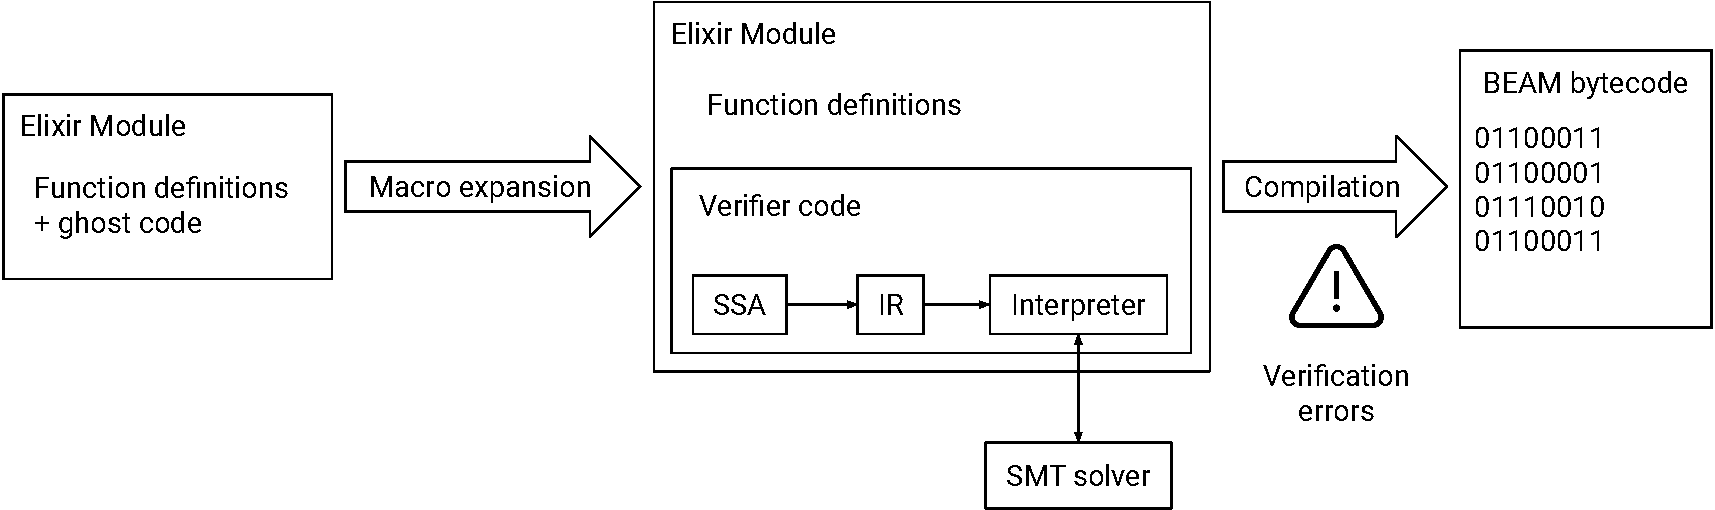
\includegraphics[width=\textwidth]{Images/Vectorial/Diagram.pdf}
      \url{https://github.com/adrianen-ucm/verixir-project}
    \end{center}
    
    \pause \bigskip

    Scope: only a subset of sequential Elixir for the moment, and partial 
    verification (i.e. not verifying termination)
  \end{frame}
  \begin{frame}{Plan}

    \begin{enumerate}
      \item \pause \acrshort*{smt} solver integration in Elixir
      \item \pause L0, a low level language close to the \acrshort*{smt} solver
      \item \pause L1, a verification \gls*{ir} for dynamically typed Elixir expressions
      \item \pause L2, a high level language that models Elixir + verification code
    \end{enumerate}
  \end{frame}
  \section{SMT Solver Integration in Elixir}
  \begin{frame}{Elixir SMT-LIB binding}
    We have developed an SMT-LIB binding for Elixir with the following features:

    \begin{itemize}
      \item \pause An SMT-LIB (subset) \gls*{dsl}
      \item \pause Different \acrshort*{smt} solvers can be easily integrated
      \item \pause Out-of-the-box support for Z3
    \end{itemize}
  \end{frame}
  \begin{frame}[fragile]{Elixir SMT-LIB binding example}
    \small
    \begin{lstlisting}[language=elixir,numbers=none,frame=none]
import SmtLib

with_local_conn do
  declare_const x: Int,
                y: Int

  assert !(
      (:x + 3 <= :y + 3) ~> (:x <= :y)
    )

  check_sat
end
      \end{lstlisting}
  \end{frame}
  \begin{frame}{The L0 language}
    \begin{itemize}
      \item \pause The lowest level language of our verification stack
      \item \pause Close to the \acrshort*{smt} solver
      \item \pause Restricted SMT-LIB + control flow + failure
    \end{itemize}
  \end{frame}
  \begin{frame}{L0 expressions syntax}
    \[
      \begin{array}{rcll}
        \Exp{0} \ni \epsilon & ::= & \skipE \\
        & | & \failE \\
        & | & \epsilon_1;\epsilon_2 \\
        & | & \localE~\epsilon \\
        & | & \addE~\varphi \\
        & | & \declareE{x} \\
        & | & \whenUnsatE{\epsilon_1}{\epsilon_2}{\epsilon_3} \\
      \end{array}
    \]

    \pause where $x \in V$ is a variable name and $\varphi \in \mathbb{F}$ is a 
    formula with many-sorted terms $t \in \mathbb{T}$
  \end{frame}
  \begin{frame}{L0 big-step operational semantics}
    Notation:
    \begin{itemize}
      \item \pause $X \subseteq V$ set of variable names
      \item \pause $\Phi \subseteq \mathbb{F}$ set of formulas
      \item \pause $\mathbb{F}(X)$ subset of $\mathbb{F}$ with free variables in $X$
      \item \pause $(X, \Phi)$ SMT solver state
      \item \pause $\BS{\epsilon}{X}{\Phi}{(X', \Phi')}$ judgement
    \end{itemize}
  \end{frame}
  \begin{frame}{L0 big-step operational semantics}
    
    \begin{prooftree}
      \AxiomC{ }
      \UnaryInfC{$\BS{\skipE}{X}{\Phi}{(X, \Phi)}$}
    \end{prooftree}

    \pause \medskip

    \begin{prooftree}
      \AxiomC{$\varphi \in \mathbb{F}(X)$}
      \UnaryInfC{$\BS{\addE~\varphi}{X}{\Phi}{(X, \Phi \cup \{\varphi\})}$}
    \end{prooftree}

    \pause \medskip

    \begin{prooftree}
      \AxiomC{$x \notin X$}
      \UnaryInfC{$\BS{\declareE{x}}{X}{\Phi}{(X \cup \{x\}, \Phi)}$}
    \end{prooftree}
    
    \pause \medskip
    
    \begin{prooftree}
      \AxiomC{$\BS{\epsilon_1}{X}{\Phi}{(X', \Phi')}$}
      \AxiomC{$\BS{\epsilon_2}{X'}{\Phi'}{(X'', \Phi'')}$}
      \BinaryInfC{$\BS{\epsilon_1;\epsilon_2}{X}{\Phi}{(X'', \Phi'')}$}
    \end{prooftree}
  \end{frame}
  \begin{frame}{L0 big-step operational semantics}
    \begin{prooftree}
      \AxiomC{$\BS{\epsilon}{X}{\Phi}{(X', \Phi')}$}
      \UnaryInfC{$\BS{\localE~\epsilon}{X}{\Phi}{(X, \Phi)}$}
    \end{prooftree}

    \pause \medskip

    \begin{prooftree}
      \AxiomC{$\BS{\epsilon_1}{X}{\Phi}{(X', \Phi')}$}
      \AxiomC{$\unsat{\Phi'}$}
      \AxiomC{$\BS{\epsilon_2}{X}{\Phi}{(X'', \Phi'')}$}
      \TrinaryInfC{$\BS{\whenUnsatE{\epsilon_1}{\epsilon_2}{\epsilon_3}}{X}{\Phi}{(X'', \Phi'')}$}
    \end{prooftree}
    
    \pause \medskip
    
    \begin{prooftree}
      \AxiomC{$\BS{\epsilon_1}{X}{\Phi}{(X', \Phi')}$}
      \AxiomC{$\neg\unsat{\Phi'}$}
      \AxiomC{$\BS{\epsilon_3}{X}{\Phi}{(X'', \Phi'')}$}
      \TrinaryInfC{$\BS{\whenUnsatE{\epsilon_1}{\epsilon_2}{\epsilon_3}}{X}{\Phi}{(X'', \Phi'')}$}
    \end{prooftree}
  \end{frame}
  \begin{frame}[fragile]{L0 Elixir implementation}
    A simple implementation in Elixir is straightforward by using our SMT-LIB binding
    \small
    \pause \bigskip

    \begin{lstlisting}[language=elixir,numbers=none,frame=none]
defmacro eval(conn, {:local, _, [e]}) do
  quote do
    conn = unquote(conn)
    :ok = push conn
    eval conn, unquote(e)
    :ok = pop conn
  end
end
    \end{lstlisting}
  \end{frame}
  \begin{frame}[fragile]{L0 Elixir example}
    \small
    \begin{lstlisting}[language=elixir,numbers=none,frame=none]
eval conn do
  declare_const :x

  when_unsat add :x != :x do
    skip # Does not reach fail
  else
    fail
  end
end
    \end{lstlisting}
  \end{frame}
  \begin{frame}[fragile]{L0 Elixir example}
    \small
    \begin{lstlisting}[language=elixir,numbers=none,frame=none]
eval conn do
  declare_const :x

  when_unsat add :x == :x do
    skip
  else
    fail # Reaches fail
  end
end
    \end{lstlisting}
  \end{frame}
  \section{Verification Intermediate Representation}
  \begin{frame}{The L1 language}
    \begin{itemize}
      \item \pause Verification \gls*{ir} 
      \item \pause It models Elixir expressions dynamically typed
      \item \pause Statements for writing verification code
    \end{itemize}
  \end{frame}
  \begin{frame}{L1 expressions syntax}
    \[
      \begin{array}{rcll}
        \Exp{1} \ni e & ::= & c \\
        & | & x \\
        & | & \andE{e_1}{e_2} \\
        & | & \orE{e_1}{e_2} \\
        & | & [] \\
        & | & [e_1~|~e_2] \\
        & | & \{e_1, \ldots, e_n\} \\
        & | & f(e_1, \ldots, e_n) \\
      \end{array}
    \]

    \pause where $c$ is a constant literal of a simple type, currently integer or 
    boolean, and $f \in \Sigma^1$ a function name
  \end{frame}
  \begin{frame}{L1 statements syntax}
    \[
      \begin{array}{rcll}
        \Stm \ni S & ::= & \skipE \\
        & | & \blockE~S \\
        & | & \havocE~x \\
        & | & S_1;S_2 \\
        & | & \assumeE~e \\
        & | & \assertE~e \\
        & | & \unfoldE~f(e_1, \dots, e_n) \\
      \end{array}
    \]
  \end{frame}
  \begin{frame}[fragile]{Built-in SMT-LIB declarations}
    Foundation to represent L1 expressions in the underlying many-sorted logic

    \pause

    \small
    \begin{verbatim}
(declare-sort Term 0)
(declare-sort Type 0)
...
(declare-const int Type)
(declare-const bool Type)
(assert (distinct int bool))
...
(declare-fun type (Term) Type)
(define-fun is_integer ((x Term)) Bool 
  (= (type x) int)
)
...
    \end{verbatim}
  \end{frame}
  \begin{frame}{Built-in L1 specifications}
    Built-in \textbf{sets} of pair/postconditions for functions to 
    model their behavior in Elixir

    \pause

    \[
      \begin{array}{l}
      \{ \isinteger{x} \wedge \isinteger{y} \}\\
      x~\texttt{+}~y\\
      \{ \\ 
      \quad\isinteger{\widehat{+}(x, y)} \wedge \\
      \quad\integervalue{\widehat{+}(x, y)} = \integervalue{x} + \integervalue{y} \\
      \}
      \end{array}
    \]

    \pause

    There could be more for other types (e.g. float)
  \end{frame}
  \begin{frame}{Translation from L1 into L0}
    \[
      \begin{array}{ll}
        \trExp{\_}{\_} : & \Exp{0} \times \Exp{1} \rightarrow \Exp{0} \times \mathbb{T}\\
        \trStm{\_} : & \Stm \rightarrow \Exp{0}
      \end{array}
    \]

    \pause

    $\trExp{\gamma}{e}$ returns a tuple $(\epsilon, t)$ where
    \begin{itemize}
      \item \pause $\epsilon$ is an L0 expression that models the semantics of $e$
      \item \pause $t$ is a term in the underlying logic to refer to the result of $e$
      \item \pause $\gamma$ models known facts by the time $e$ is evaluated
    \end{itemize}
  \end{frame}
  \begin{frame}{Translation of L1 lists}
    \[
      \begin{array}{l}
      \trExp{\_}{[]} \equiv (
        \skipE, \mathit{nil}
      )\\
      \trExp{\gamma}{[e_1~|~e_2]} \equiv (\epsilon_1;\epsilon_2;\epsilon, t)\\
        \qquad \textbf{where } (\epsilon_1, t_1) = \trExp{\gamma}{e_1}\\ 
        \qquad \phantom{\textbf{where }} (\epsilon_2, t_2) = \trExp{\gamma}{e_2}\\ 
        \qquad \phantom{\textbf{where }} t = \mathit{cons}(t_1, t_2)\\ 
        \qquad \phantom{\textbf{where }} \epsilon = \left[
          \begin{array}{l}
            \addE~\isnelist{t};\\
            \addE~\mathit{hd}(t) = t_1;\\
            \addE~\mathit{tl}(t) = t_2\\
          \end{array}
        \right]
      \end{array}
    \]
  \end{frame}
  \begin{frame}{Translation of L1 lists example}
    \[
      \begin{array}{l}
      \trExp{\gamma}{[2, x]} \equiv (\epsilon, \mathit{cons}(2, \mathit{cons}(\hat{x}, \mathit{nil})))\\
      \qquad \textbf{where } \epsilon = \left[ 
      \begin{array}{l}
      \addE~\mathit{is\mbox{-}integer}(\mathit{integer\mbox{-}lit}(2));\\
      \addE~\mathit{integer\mbox{-}value}(\mathit{integer\mbox{-}lit}(2)) = 2;\\
      \addE~\isnelist{\mathit{cons}(\hat{x}, \mathit{nil})};\\
      \addE~\mathit{hd}(\mathit{cons}(\hat{x}, \mathit{nil})) = \hat{x};\\
      \addE~\mathit{tl}(\mathit{cons}(\hat{x}, \mathit{nil})) = \mathit{nil};\\
      \addE~\isnelist{\mathit{cons}(2, \mathit{cons}(\hat{x}, \mathit{nil}))};\\
      \addE~\mathit{hd}(\mathit{cons}(2, \mathit{cons}(\hat{x}, \mathit{nil}))) = 2;\\
      \addE~\mathit{tl}(\mathit{cons}(2, \mathit{cons}(\hat{x}, \mathit{nil}))) = \mathit{cons}(\hat{x}, \mathit{nil});\\
      \end{array}
      \right]
      \end{array}
    \]
  \end{frame}
  \begin{frame}[fragile]{L1 Elixir implementation}
    Our implementation is quite direct from the formalization

    \pause
    \small
    \begin{lstlisting}[language=elixir,numbers=none,frame=none]
def tr_exp(_, [{:|, _, [h, t]}]) do
  {h, h_sem} = tr_exp(_, h)
  {y, t_sem} = tr_exp(_, t)
  t = 
    quote(do: :cons.(unquote(h), unquote(t)))

  { t, quote do
    unquote(h_sem)
    unquote(t_sem)
    add :is_nonempty_list.(unquote(t))
    add :hd.(unquote(t)) == unquote(h)
    add :tl.(unquote(t)) == unquote(t)
  end }
end
    \end{lstlisting}
  \end{frame}
  \begin{frame}[fragile]{L1 Elixir example}
    \small
    \begin{lstlisting}[language=elixir,numbers=none,frame=none]
import Boogiex

with_local_env do
  assert (false or 2) === 2
  assert elem({1, 2, 3}, 0) === 1
  assert true or true + true

  havoc x
  assert x === x
  assert not (x !== x)
end
    \end{lstlisting}
  \end{frame}
  \section{Elixir Code Verification}
  \begin{frame}{The L2 language}
    \begin{itemize}
      \item \pause The highest level language of our verification stack
      \item \pause Elixir (subset) + ghost verification code
    \end{itemize}
  \end{frame}
  \begin{frame}{L2 expressions syntax}
    \[
      \begin{array}{rcll}
      \Exp{2} \ni E & ::= & e \\
      & | & P = E \\
      & | & \emptyE \\
      & | & E_1; E_2 \\
      & | & \caseE~E~\doW \\
      & & \quad P_1~\whenE~f_1 \rightarrow E_1 \\
      & & \quad \vdots\\
      & & \quad P_n~\whenE~f_n \rightarrow E_n \\
      & & \Wend \\
      & | & \ghostE~\doW~S~\Wend \\
      \end{array}
    \]

    \pause where $P, P_1, \dots P_n$ are patterns:
    \[
      \Pat \ni P ::= c \mid x \mid [\:] \mid [P_1 \mid P_2] \mid \{ P_1, \ldots, P_n \}
    \]
  \end{frame}
  \begin{frame}{Translation from L2 into L1}
    \[
      \begin{array}{ll}
        \trEXP{\_} : \Exp{2} \rightarrow [\Stm \times \Exp{1}]\\
        \trMatch{\_}{\_} : \Exp{1} \times \Pat \rightarrow \Exp{1}
      \end{array}
    \]

    \pause $\trEXP{E}$ generates a sequence of pairs $(S, e)$ where
    \begin{itemize}
      \item \pause $S$ is an L1 statement that models the semantics of $E$
      \item \pause $e$ is an L1 expression that represents the result to which $E$ is evaluated
      \item \pause Each pair corresponds to an execution path
    \end{itemize}
  \end{frame}
  \begin{frame}{Translation of L2 lists pattern matching}
    $\trMatch{e}{P}$ returns an L1 expression that is a $\mathit{boolean}$ 
    term and is evaluated to $\true$ if and only if $e$ matches $P$

    \pause 

    \[
      \begin{array}{l}
        \trMatch{e}{[P_1\mid P_2]} = \\
        \qquad\textit{is-nelist}(e)~\mathbf{and}\\
        \qquad\trMatch{\textit{hd}(e)}{P_1}~\mathbf{and}\\
        \qquad\trMatch{\textit{tl}(e)}{P_2}
      \end{array}
    \]
  \end{frame}
  \begin{frame}{Translation of L2 pattern matching expressions}
    \[
      \begin{array}{l}
      \trEXP{P = E} = [(S_1;S_1',e_1), \dots, (S_n;S_n', e_n)] \\
      \qquad 
      \begin{array}{ll}
      \textbf{where} & [(S_1,e_1),\dots,(S_n, e_n)] = \trEXP{E} \\
      & \{y_1, \ldots, y_m\} = \mathit{vars}(P) \\
      & \forall i \in \{1..n\}: S_i' = \left(
      \begin{array}{l}
      \assertE~\trMatch{e_i}{P};\\
      \havocE~y_1;\\
      \vdots\\
      \havocE~y_m;\\
      \assumeE~e_i ~\texttt{===}~ P\\
      \end{array}
      \right)
      \end{array}
      \end{array}
    \]
  \end{frame}
  \begin{frame}{Verifying user-defined functions}
    A single clause of a function with arity $n$:

    \[
    \mathit{def} \equiv \left(\{ p \}  \quad (P_1, \dots, P_n)~B \quad \{ q \} \right)
    \]

    \pause where $p \in \Exp{1}$ and $q \in \Exp{1}$ denote a specified precondition and a
    postcondition, $P_1, \dots, P_n$ are the parameter patterns and $B \in \Exp{2}$
    is its defined body

    \pause \medskip

    Clauses of a function $f$ with arity $n$:

    \[
      \Defs{f/n} = (\mathit{def}_1,\dots,\mathit{def}_k)
    \]
  \end{frame}
  \begin{frame}{Verifying user-defined functions}
    \begin{enumerate}
      \item \pause Transform the function definition clauses into an L2 case 
        expression with the parameter variables free and a trivial branch
      \item \pause Apply Static Single-Assignment to allow rebinding variables
      \item \pause Translate it into the corresponding execution paths in our \gls*{ir}
      \item \pause Translate each path into an L0 statement
      \item \pause Verify them independently of each other
    \end{enumerate}

    \pause \textbf{Note:} our formalization does not address currently the verification 
    of user-defined function invocations (i.e. their specifications and body unfolding),
    but our implementation does it by automatically generating ghost code.
  \end{frame}
  \begin{frame}[fragile]{L2 Elixir implementation}
    Again, our implementation is quite direct from the formalization

    \pause
    \small
    \begin{lstlisting}[language=elixir,numbers=none,frame=none]
def tr_match({:|, _, [p1, p2]}, e) do
  tr_1 = 
    tr_match(p1, quote(do: hd(unquote(e))))
  tr_2 = 
    tr_match(p2, quote(do: tl(unquote(e))))

  quote(do:
    is_list(unquote(e)) and 
    unquote(e) !== [] and
    unquote(tr_1) and unquote(tr_2)
  )
end
    \end{lstlisting}
  \end{frame}
  \begin{frame}[plain,c]{L2 Elixir example}
    \begin{center}
      \Huge Live demo
    \end{center}
  \end{frame}
  \section{Conclusions}
  \begin{frame}{Conclusions}
    \begin{itemize}
      \item \pause We have developed a framework for Elixir code verification across several areas (i.e. \acrshort*{smt} solver integration, verification \gls*{ir} and code verification)
      \item \pause Future work may address concurrent code and total verification
      \item \pause Also, we have left several improvements on the way:
      \begin{itemize}
        \item \pause More of the SMT-LIB standard and \acrshort*{smt} solvers support
        \item \pause Extend our \gls*{ir} to model more Elixir value types and built-in functions
        \item \pause Extend the Elixir subset to verify (e.g. pin operator and higher-order)
        \item \pause The current implementation is in an early proof of concept stage
      \end{itemize}
    \end{itemize}
  \end{frame}
  \appendix
  \maketitle
\end{document}
